\documentclass[10pt,a4paper]{article}
\usepackage[utf8]{inputenc}
\usepackage{amsmath}
\usepackage{amsfonts}
\usepackage{amssymb}

\usepackage[pdftex]{hyperref}
\usepackage{graphicx}


\author{Isaque Vieira Machado Pim \\
Fundação Getúlio Vargas \\
EMAp}
\title{Relatório - Modelagem SARIMA para consumo elétrico}
\begin{document}
\maketitle

\section{Introdução}
Relatório referente a primeira avaliação da disciplina de Séries Temporais, ministrada pelo professor Eduardo Fonseca Mendes. Aqui analisamos as séries mensais de consumo elétrico do estado do Espírito Santo. Os dados vão de janeiro de 2004 a junho de 2021, e estão disponíveis em \href{https://www.epe.gov.br/pt/publicacoes-dados-abertos/publicacoes/consumo-de-energia-eletrica}{\textbf{neste hiperlink}}. Os dados estão dispostos de maneira conjunta e desagregada, separado nas classes: Residencial, Comercial, Industrial, Cativo e Outros. 

\begin{figure}[h]
\centering
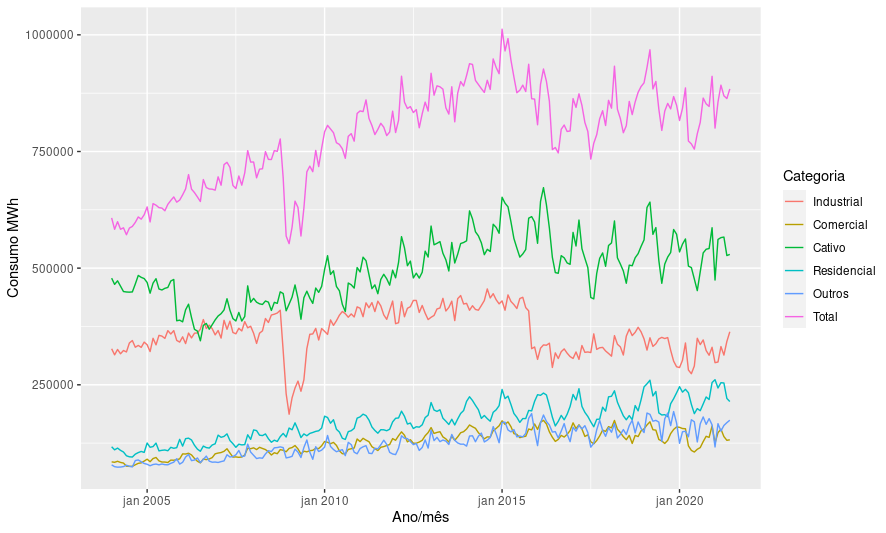
\includegraphics[width=.8 \linewidth]{../tudo.png} 
\caption{Plot do consumo total e classes separadas.}
\end{figure}

De cara já podemos identicar dois momentos ímpares na série: Um entorno de 2009, e outro em torno de 2016, ambos afetando fortemente o setor industrial. As \href{https://www.agazeta.com.br/es/economia/conheca-as-10-maiores-empresas-que-atuam-no-espirito-santo-1220}{\textbf{maiores empresas}} atuando no Espírito Santo são: Petrobras, Vale e  ArcelorMittal.\\ 
 Buscando pro momentos de crise no país e, em específico, no setor siderurgico e petrolífero, encontramos rapidamente que esses dois momentos em destaque tem nome:
\href{https://www1.folha.uol.com.br/fsp/dinheiro/fi1012200837.htm}{\textbf{Crise 2009}},  \href{https://www.manufaturaemfoco.com.br/a-crise-que-abalou-a-siderurgia/#:~:text=A\%20ind\%C3\%BAstria\%20sider\%C3\%BArgica\%20brasileira\%20viveu,j\%C3\%A1\%20cr\%C3\%ADtico\%20ano\%20de\%202015.}{\textbf{Crise 2016}}\\
Esses fatores serão levados em conta na modelagem. A modelagem será feita toda em R. A versão utilizada é a 4.1.1. Os códigos virão em anexo com o relatório.

\section{Preliminares}
Antes de rodar os scripts que fazem a análise, o script R \textbf{extract.r} deve ser executado para gerar a variável "ES", contendo todas as séries em questão. Outro script que vem junto e é auxiliar é o \textbf{visualize.r}, que faz alguns plots informativos sobre a série, um deles marcando os dois períodos de crise no setor industrial na série agregada. \textbf{packages.r} contém as libraries usadas nos scripts.
\section{Modelagem da série agregada}

A modelagem da série agregada será feita de duas maneiras: Uma determinística e outra através de um modelo SARIMA.

\subsection{Determinístico}

O método que escolhi foi ajustar um modelo regressivo linear junto com \textit{dummy variables} para modelar tendência e sazonalidade, respectivamente.O script referente a esta parte é \textbf{Regression.r}. A regressão possui duas intervenções para ajudar a sazonalidade se ajustar melhor, referente aos dois períodos de crise mencionados. Um atua como um choque constante pelo período, e o outro como uma spline, modificando a inclinação da reta durante o período.Para tentar regular um pouco a variância crescente, apliquei uma tranformação logaritmica no valor da série, mesmo com a transformação feita. O fit da regressão junto com a sazonalidade é bom ($R^2 > 0.9$), como o esperado depois de duas incisões precisas, mas isso não pode dizer muito sobre a poder preditivo do modelo. Claramente a precisão não foi boa, e um dos modivos seŕa até discutido mais a frente no trabalho, a regressão não conseguiu absorver o aumento da variância no final da série. Outro ponto é que pandemia não foi levada em conta, mas é um evento futuro ao treino. Seguem plots da série, das linhas de regressão, e do modelo ajustado. \newpage

\begin{figure}[h]
\centering
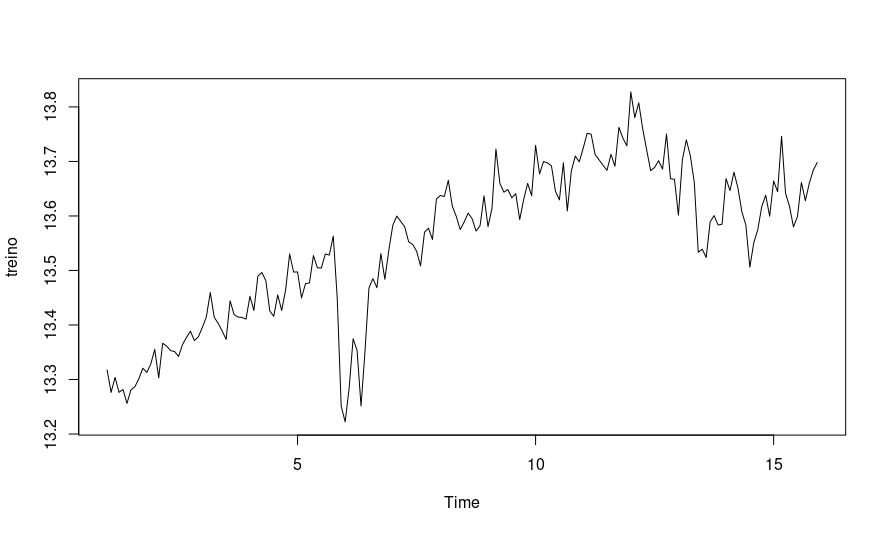
\includegraphics[width=.8 \linewidth]{../regressao_pura.png} 
\caption{Dados usados para treino.}
\end{figure}

\begin{figure}[h]
\centering
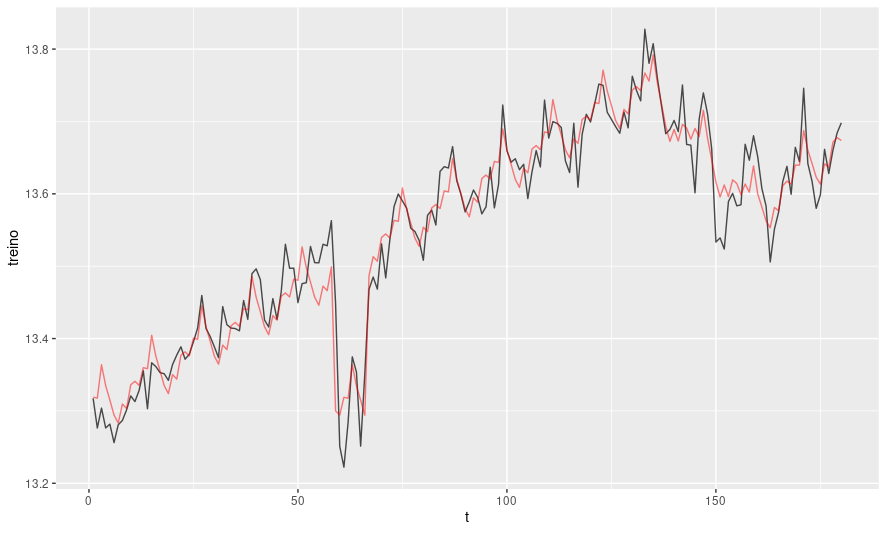
\includegraphics[width=.8 \linewidth]{../regressao_fitted_model.png} 
\caption{Modelo fitado}
\end{figure}

\begin{figure}[h]
\centering
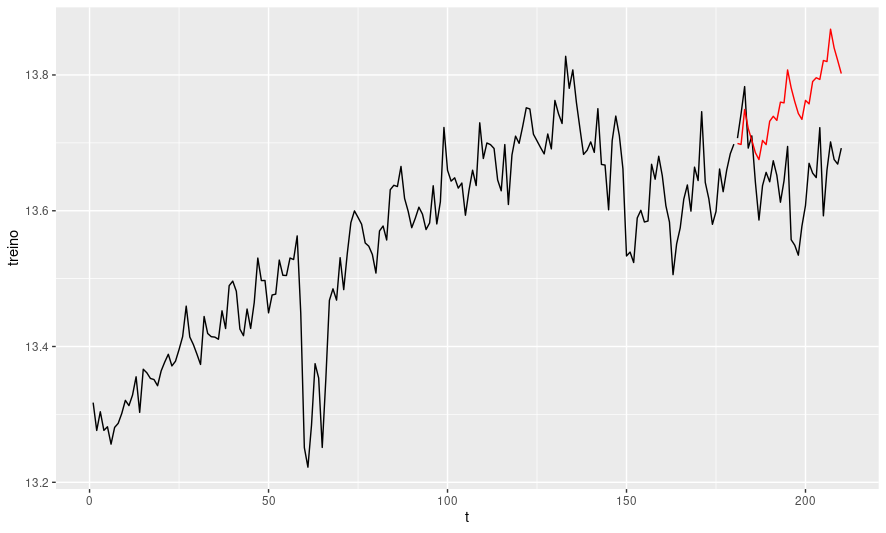
\includegraphics[width=.8 \linewidth]{../predicted.png} 
\caption{Resultado da predição em vermelho}
\end{figure}

\newpage

\subsection{SARIMA}

A modelagem SARIMA se encontra no script \textbf{SARIMA.r}. Duas linhas de ideia foram executadas ali. Já sabemos que essa série tem uma grande descontinuidade em 2009. A primeira tentativa é uma regressão com erros SARIMA, a regressão sendo apenas para a primeira descontinuidade.Lembrando que estamos trabalhando com o log da série. A segunda é descartar o pedaço da série que vem antes do fim da crise de 2009. Os resultados foram mais satisfatórios para o segundo caso. O erro quadrático médio para o modelo sem o descarte de parte da série foi de 0.1029459. Para o segundo caso o erro quadrático médio foi de 0.01525633. A escolha do modelo 1 foi feita automaticamente pelo auto.arima por motivos práticos. O modelo 2 foi selecionado pelo estudo da ACF e PACF da série. Seguem as imagens geradas por script.

\begin{figure}[h]
\centering
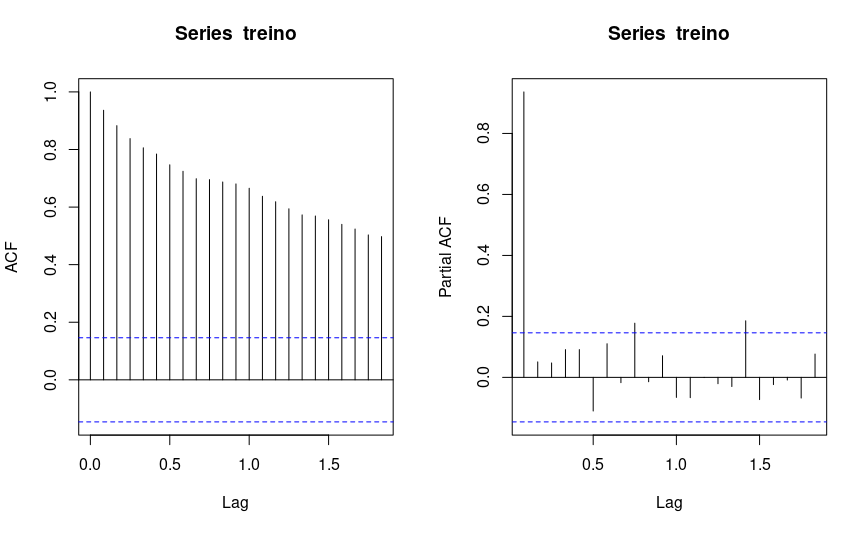
\includegraphics[width=.8 \linewidth]{../trendSARIMA.png} 
\caption{ACF e PACF da série}
\end{figure}

\begin{figure}[ht]
\centering
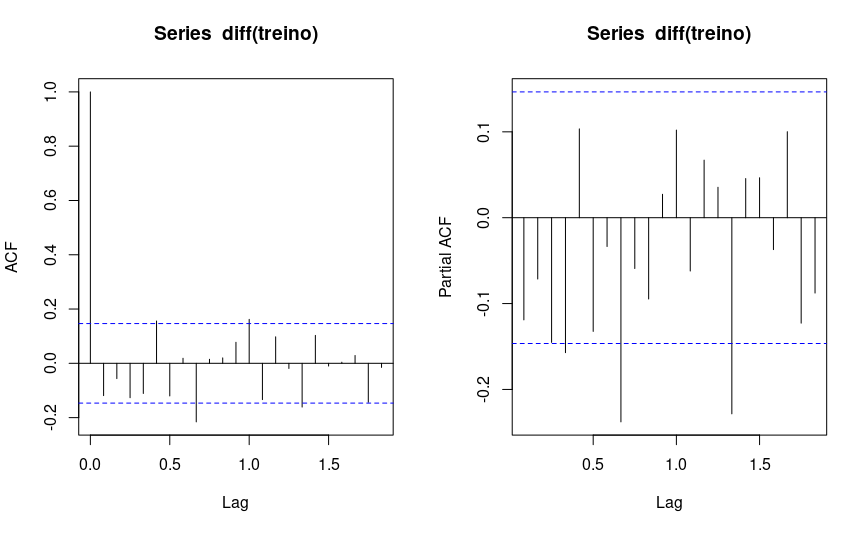
\includegraphics[width=.8 \linewidth]{../trendDIFF.png} 
\caption{ACF e PACF da série diferenciada}
\end{figure}
A ACF da série de treino indica existe uma tendência pelo decaimento lento. Diferenciando a série conseguimos ver que esse decaimento lento some. A série diferenciada possui elementos com correlação mais alta nos lags: 5,8,12,16,21. A PACF tem seus maiores picos nos lags 8 e 16. O ACF não indica presença de componente auto-regressiva nem  auto-regressiva sazonal, um dos picos na ACF ocorrerem no 12 pode indicar uma componente MA sazonal, assim como picos mais significativos na PACF nos estimulam a adicionar componetes MA em geral. Diferenciação sazonal para captar entre como opcão. Os modelos para teste ficam do tipo $SARIMA(0,1,q)(0,D,Q)_{12}$, com $D = \text{0 ou 1}$ $1 \leq q,Q \leq 3$. O modelo escolhido como melhor foi o $SARIMA(0,1,1)(0,1,1)_{12}$. O único problema é que ao final no lugar de um pico há uma queda, que deve ocorrer supostamente pela pandemia.

\begin{figure}[h]
\centering
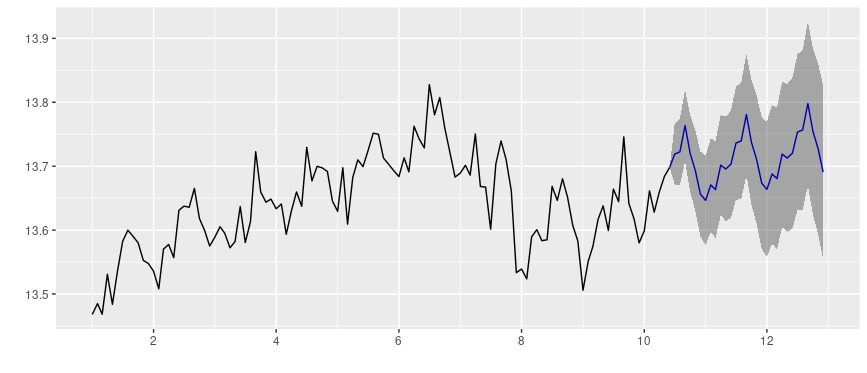
\includegraphics[width=.8 \linewidth]{../confidenceSARIMA.png} 
\caption{Intervalos de confiança e valores preditos}
\end{figure}

\begin{figure}[ht]
\centering
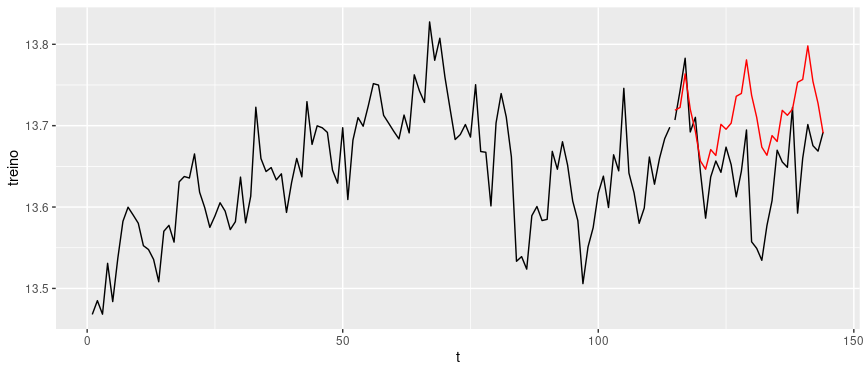
\includegraphics[width=.8 \linewidth]{../fittedSARIMA.png} 
\caption{Comparação com a série original. Valores preditos em vermelho}
\end{figure}


\section{Impacto da Pandemia}

Agora vamos analisar o impacto da pandemia nas séries desagregadas. Para isso vamos utilizar modelos SARIMA. As séries desagregadas são mais bem comportadas (com exceção da indústria), então a única variável exógena será a própria pandemia. As análises estarão no arquivo \textbf{parte2.r} com o mesmo nome da respectiva classe. Vou aqui apenas dispor o parâmetro que veio da regressão. Com algumas poucas exceções, a maioria dos modelos foi fitada usando auto.arima(). Os cuidados tiverem que ser analisados nos resultados do auto.arima e na definição da série a ser modelada. A série industrial e a cativa tiveram seus anos inciais cortados para melhor modelagem. Os resultados vieram colhendo os parametros e valores do summary() e invertendo para o original e assim ter uma noção do baque inicial causado pela pandemia.

\begin{itemize}
\item Residencial - Diminuição de 5000 MWh no início da pandemia. Aumento Relativo: -2\%
\item Comercial - Diminuição de 25000 MWh no início da pandemia. Aumento Relativo: -16\%
\item Cativo - Diminuição de 36000 MWh no início da pandemia. Aumento Relativo: -6\%
\item Outros - Diminuição de 24000 MWh no início da pandemia. Aumento Relativo: -16\%
\item Industrial - Aumento de 10000 MWh no início da pandemia. Aumento Relativo: +3\%
\end{itemize}. 

Comércio e outros(setor público, por exemplo), foram os único com aumento relativo significante, o que encaixa com a realidade. O industrial apresentou esse aumento relativo por estar voltando de uma crise no início de 2020.

\section{Discussão e desafios enfrentados}

Durante o desenvolvimento do trabalho tive grande suporte no textbook online Forecasting: Principles and Practice, que apresenta de maneira introdutória modelagem de séries. A série estudada no trabalho foi complicada devido as perturbações grandes de crises que de fato acontencem na vida real, mas para esse caso as regressões conseguiram dar conta. Outro ponto foi a variância crescente ao longo do tempo, e que não consegui corrigir com as transformações de Box.Cox. Também a análise de ACF e PACF segue um pouco diferente dos livros. Não existe um pico claro em determinado lag, mas muitos picos médios espalhados em lags distintos. A análise de parâmetros p e q para o modelo foram várias tentativas alternando entre os lags que mais se destacavam. Algumas vezes no trabalho o auto.arima encontrou raízes fora do círculo unitário (talvez pela variância não corrigida), o que precisou de uma análise mais profunda das correlações naquele caso para encontrar um modelo.
\end{document}






